%%%%%%%%%%%%%%%%%%%%%%%%%%%%%%%%%%%%%%%%%%%%%%%%%%%%%%%%%%%%%%%%%%%%%%%
%
%   Presentation of Beamer UNL Theme
%   Beamer Presentation by Chris Bourke
%
%%%%%%%%%%%%%%%%%%%%%%%%%%%%%%%%%%%%%%%%%%%%%%%%%%%%%%%%%%%%%%%%%%%%%%%
%% Make tables with set width
\documentclass{beamer}
%% Be able to use subfigure
%\usepackage{caption}
\usepackage{subcaption}
\captionsetup{compatibility=false}

\usetheme[hideothersubsections]{UNLTheme}


\title[HAL - Protein]{HIERARCHICAL ACTIVE LEARNING (HAL) APPLICATION TO MITOCHONDRIAL DISEASE PROTEIN DATASET}
\author{James Duin} %
\institute{University of Nebraska--Lincoln \\ Master's Thesis}
\date{Spring 2017 \\ \href{mailto:jamesdduin@gmail.com}{\color{blue}{\texttt{jamesdduin@gmail.com}}}}

\begin{document}
%{% open a Local TeX Group
%\setbeamertemplate{sidebar}{}
\begin{frame}    % slide 1
    \titlepage
\end{frame}
%}% end Local TeX Group





%1. Introduction: define problem, present a “car-
%rot”, put in context, and give outline
%2. Body: high level summary of key results
%3. Technicalities: more depth into a key result
%4. Conclusion: review key results, wrap up, give future work


%The Introduction
%• Define the Problem
%– minimize use of terminology
%– use pictures/examples/props if possible
%• Motivate the audience (give a “carrot”) – why is problem important?
%– how does it fit into larger picture?
%– what are applications?
%• Discuss related work
%– table useful (mention authors and dates)
%• Succinctly state contributions of your work • Provide a road-map (outline)


\section{Introduction}
\begin{frame}
    \frametitle{Introduction}   % slide 2
    \framesubtitle{}
    \begin{itemize}
      \item Identify the source of mutations which give rise to mitochondrial disease
      \item Leigh Syndrome, Leber’s Hereditary Optic Neuropathy %- blindness %- respiratory failure
      \item Hierarchically labeled according to location in mitochondria
      \item Coarse-grained: learning labels near the root of the tree
      \item Fine-grained: learning labels towards the leaf nodes
      \item Learn mitochondrion concept (coarse) by combining classifiers for each target compartment (fine)
    \end{itemize}
\end{frame}
\begin{frame}
    \frametitle{Introduction}     % slide 3
    \framesubtitle{Related Work}
    \begin{itemize}
      \item \textbf{Active learning}: copious unlabeled data, cost associated with acquiring labels,
      yields best classifier for a given cost, or best for minimal cost
      \item Previous work in text classification and and rich media indexing use hierarchies of
      labels to improve fine-level classification (McCallum et al. 1998, Jiang et al. 2013)
      \item Previous work in named entity recognition to target fine-grained entity categories (Fleischman et al. 2002)
      \item \textbf{First, investigation of active learning in a hierarchical setting, approach
      shown to find best classifier for a budget regardless of varying label acquisition cost}
    \end{itemize}
\end{frame}
\begin{frame}
    \frametitle{Introduction}    % slide 4
    \framesubtitle{}
\par Outline:
\begin{itemize}
  \item Machine Learning
  \item Active Machine Learning
  %\item Evaluating Classifier Performance
  \item Hierarchical Protein Dataset
  \item Coarse-grained vs Fine-grained Trade Off
  \item Active over-labeling algorithms
%  \item HAL and BANDIT
%  \item Hierarchical Active Learning
%  \item Dynamically Adapting Purchase Proportions
  \item Application to Protein Dataset
  \item Experimental Results
%  \item Training and Testing Coarse-grained and Fine-grained Classifiers
%  \item SVM and Logit Classifier Performance
%  \item Active vs Passive Curve Analysis
%  \item Plots for Fine Fixed Ratio Results
%  \item BANDIT Approach Results
%  \item Conclusions and Future Work
\end{itemize}
\end{frame}









\section{Background}
\begin{frame}
    \frametitle{Machine Learning}
    \framesubtitle{}
    \begin{figure}[!htb]
        \begin{flushleft}
        \par INPUT: labeled data
        \par OUTPUT: learned hypothesis used to predict new instances
        \end{flushleft}
%   \begin{itemize}
%      \item INPUT: labeled data
%      \item OUTPUT: learned hypothesis used to predict new instances
%    \end{itemize}
%    \vspace*{-\baselineskip}
%    \vspace*{-\baselineskip}
        \centering
        \par $h_\theta(x)$, for fixed $\theta_0$ and $\theta_1$ line coefficients
    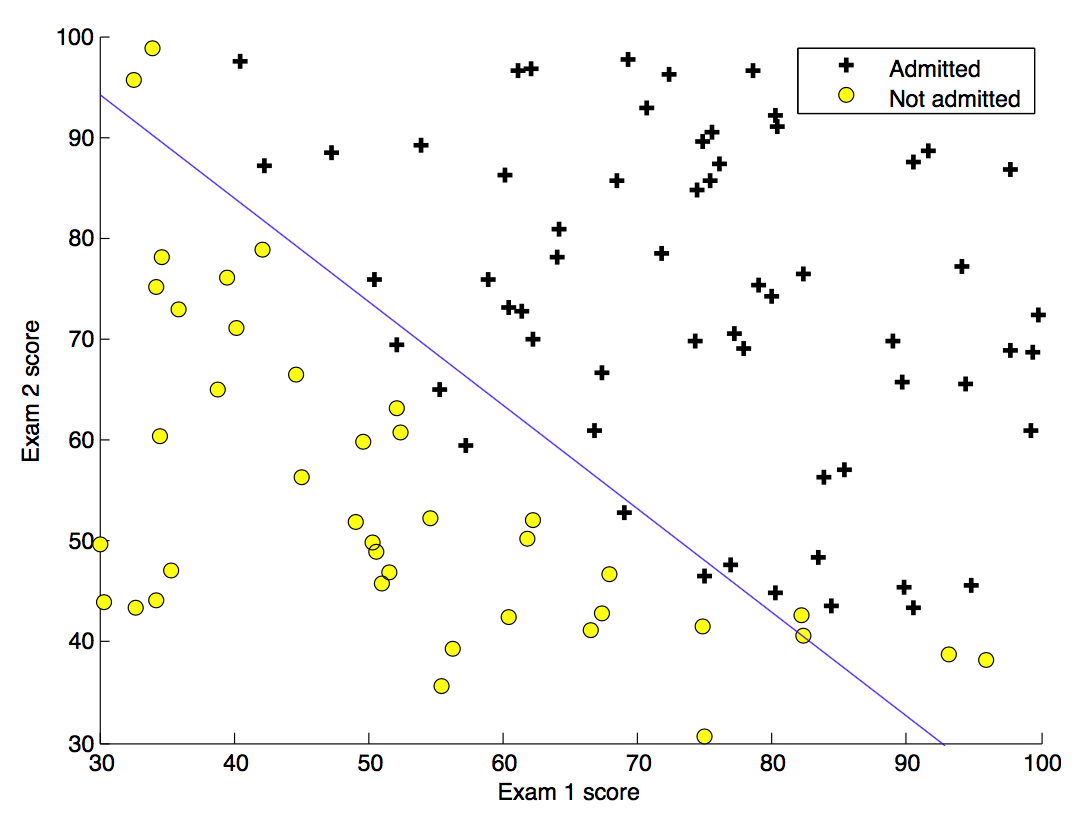
\includegraphics[width=0.70\columnwidth]{fig/ML_labels}
        \label{fig:ML_labels}
    \end{figure}
\end{frame}
\begin{frame}
    \frametitle{Machine Learning}
    \framesubtitle{Cost Function}
    \begin{figure}[!htb]
        \centering
    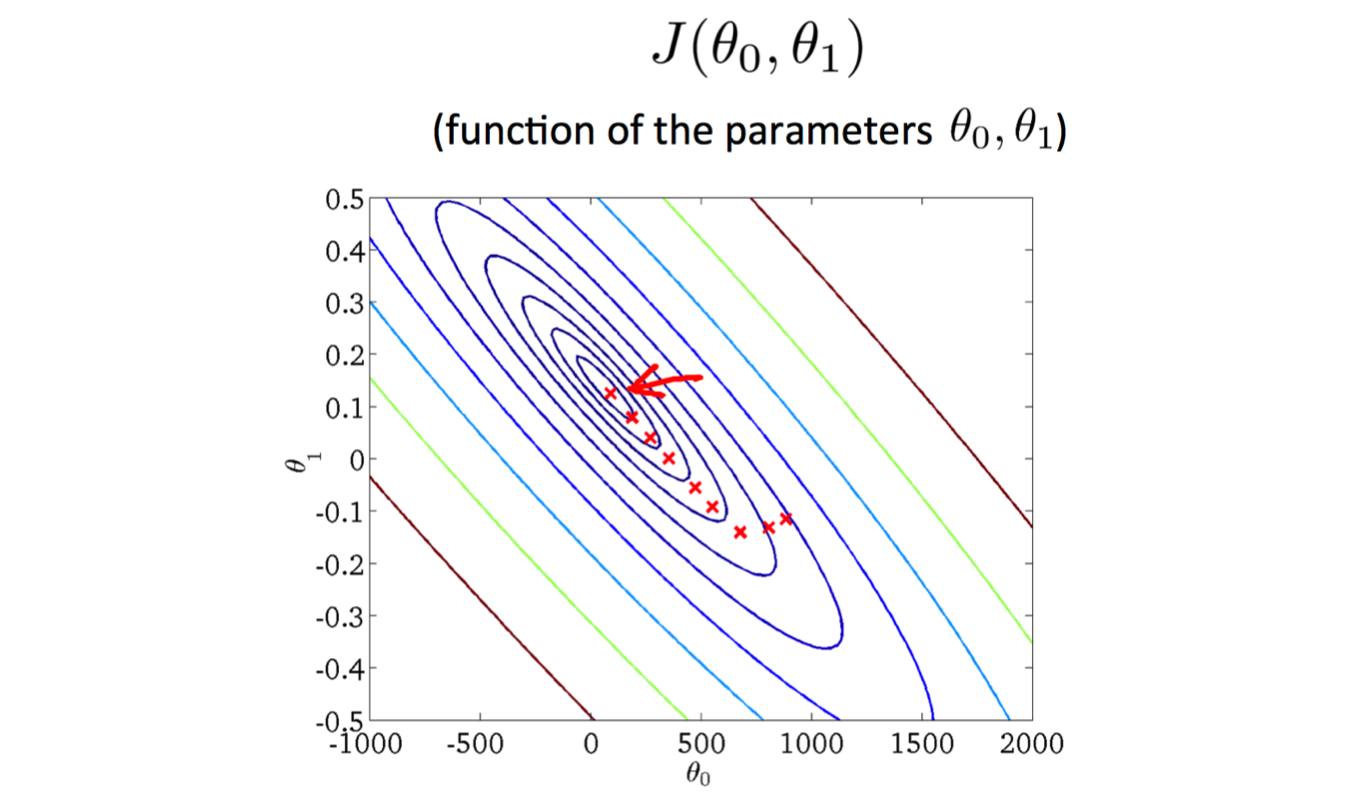
\includegraphics[width=1.0\columnwidth]{fig/ML2}
        \label{fig:ML2}
    \end{figure}
\end{frame}
\begin{frame}
    \frametitle{Machine Learning}
    \framesubtitle{Support Vector Machine (SVM)}
    \par And SVM constructs a line, plane or hyperplane
    that separates the features with the greatest margin.

    \begin{figure}[!htb]
        \centering
    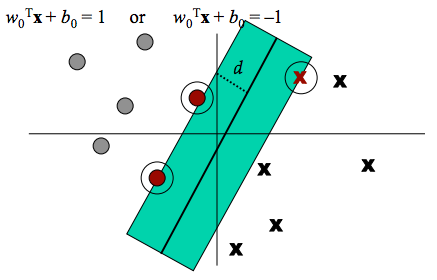
\includegraphics[width=0.9\columnwidth]{fig/SVM1}
        \label{fig:SVM1}
    \end{figure}
\end{frame}
\begin{frame}
    \frametitle{Machine Learning}
    \framesubtitle{Support Vector Machine (SVM)}
    \par The greater the functional margin the lower the
    generalization error of the classifier
    \begin{figure}[!htb]
        \centering
    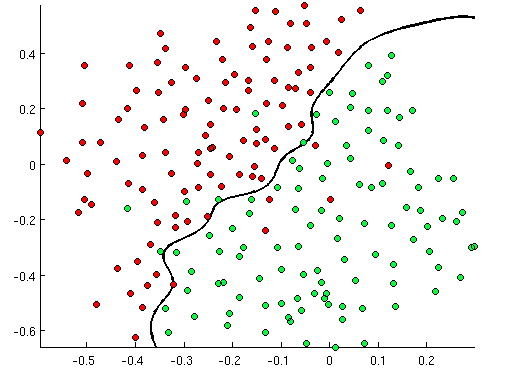
\includegraphics[width=0.8\columnwidth]{fig/RBFSVM1}
        \label{fig:RBFSVM1}
    \end{figure}
\end{frame}
\begin{frame}
    \frametitle{Machine Learning}
    \framesubtitle{Support Vector Machine (SVM)}
    \par Kernel functions implicitly map inputs into high-dimensional feature spaces
    \begin{figure}[!htb]
        \centering
    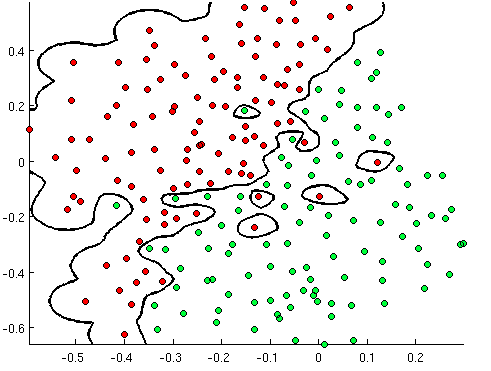
\includegraphics[width=0.8\columnwidth]{fig/RBFSVM2}
        \label{fig:RBFSVM2}
    \end{figure}
\end{frame}
\begin{frame}
    \frametitle{Machine Learning}
    \framesubtitle{Logistic Regression (Logit)}
        \par Logistic Regression (Logit) estimates the probability of a binary response,
    learns coefficients \textbf{w} of the input vector \textbf{x} and passes dot product through sigmoid function. (Maximum likelihood learning)
         \begin{figure}[!htb]
        \centering
    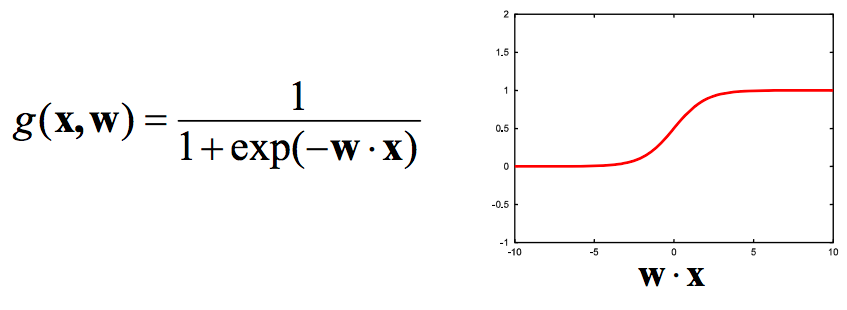
\includegraphics[width=1.0\columnwidth]{fig/logit1}
        \label{fig:logit1}
    \end{figure}
%    $\begin{aligned}
%h_{\theta}(x) = g(\theta \cdot x) \\
%g(z) = \frac{1}{1+e^{-z}}
%\end{aligned}$
\end{frame}



%\begin{frame}
%    \frametitle{Machine Learning}    % slide 5
%    \framesubtitle{}
%\begin{itemize}
%  \item Machine learning (ML) algorithms are defined as computer programs that learn from experience E
%with respect to some class of tasks T and performance measure P, if their performance at
%tasks in T, as measured by P, improves with experience E - (Mitchell 1997).
%  \item Support Vector Machine (SVM) - Uses support vectors and kernel functions %which give measures of similarity between data instances to output classification labels
%  \item Logistic Regression (Logit) - Uses logistic function %to output classification labels
%\end{itemize}
%\end{frame}
\begin{frame}
    \frametitle{Active Machine Learning}     % slide 6
    \framesubtitle{}
\begin{itemize}
  \item The learner queries an \textbf{oracle} or \textbf{supervisor} which labels the data at a certain cost
  \item Active learning solicits new instances that can maximally improve performance of the learned classifier
  \item Learns the best performing classifier for the minimal amount of labeling cost,
  or for a given purchase budget
  \item Acquires labels for each level of the hierachy at a certain cost, spends according to a purchase budget
\end{itemize}
\end{frame}
%\begin{frame}
%    \frametitle{Evaluating Classifier Performance}
%    \framesubtitle{Confusion Matrix}     % slide 7
%%    \begin{itemize}
%%      \item Divide data into train and a test set. Analyze test set with the following values:
%\par Divide data into train and a test set. Analyze test set with the following values:
%      \begin{itemize}
%      \item True-Negatives ($T_n$): Correctly classified negatives
%      \item False-Negatives ($F_p$): Incorrectly classified negatives
%      \item False-Positives ($F_n$): Incorrectly classified positives
%      \item True-Positives ($T_p$): Correctly classified positives
%%    \end{itemize}
%    \end{itemize}
%    \par Example of a confusion matrix for a test set with $100$ negatives and $50$ positives:
%    \begin{table}[H]
%    \centering
%    %\caption{Example of a confusion matrix, with $100$ negative and $50$ positive instances in the test set}
%    \label{tab:confEx}
%    \begin{tabular}{|l||l|}\hline
%    conf ($T_n$/$F_n$) & conf ($F_p$/$T_p$) \\ \hline
%    90 & 10 \\ \hline
%    20 & 30 \\ \hline
%    \end{tabular}
%    \end{table}
%\end{frame}
%\begin{frame}
%    \frametitle{Evaluating Classifier Performance}  % slide 8
%    \framesubtitle{Precision and Recall}
%    Precision is a measure of result relevancy:
%    \begin{equation}
%    \label{eq:precision}
%    \begin{aligned}
%    P = \frac{T_p}{T_p+F_p}
%    \end{aligned}
%    \end{equation}
%    Recall is a measure of how many truly relevant results are returned:
%    \begin{equation}
%    \label{eq:recall}
%    \begin{aligned}
%    R = \frac{T_p}{T_p+F_n}
%    \end{aligned}
%    \end{equation}
%\end{frame}
%\begin{frame}
%    \frametitle{Evaluating Classifier Performance}  % slide 9
%    \framesubtitle{F-Measure}
%    The F-measure or F1-measure (F1) is the harmonic mean of precision and recall:
%    \begin{equation}
%    \label{eq:fmes}
%    \begin{aligned}
%    F1 = 2\cdot \frac{P \cdot R}{P+R}
%    \end{aligned}
%    \end{equation}
%\end{frame}
%\begin{frame}
%    \frametitle{Evaluating Classifier Performance}  % slide 10
%    \framesubtitle{ROC - PR curves}
%    \begin{figure}[!htb]
%        \centering
%        \begin{subfigure}[t]{0.5\textwidth}
%            \centering
%            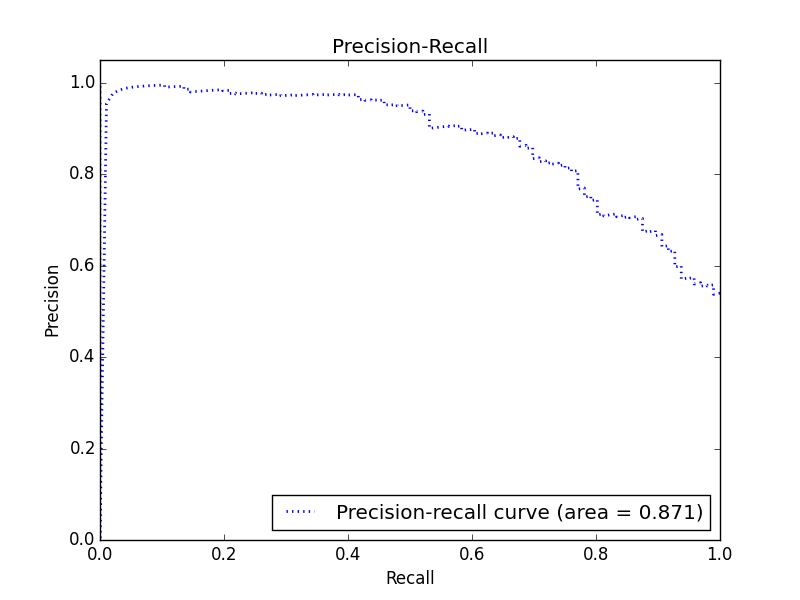
\includegraphics[width=\textwidth]{fig/Psv_1_2_fine_PR}
%            \caption{PR curve.}
%        \end{subfigure}%
%        ~
%        \begin{subfigure}[t]{0.5\textwidth}
%            \centering
%            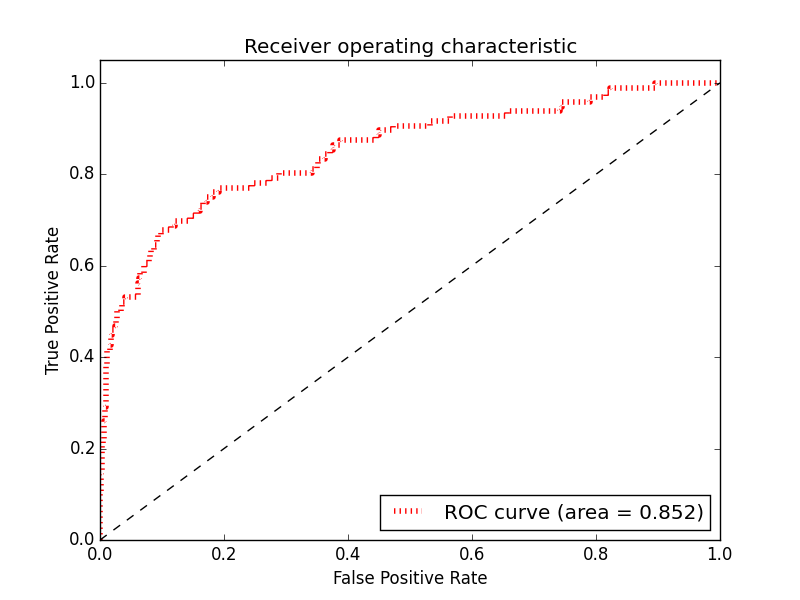
\includegraphics[width=\textwidth]{fig/Psv_1_2_fine_ROC}
%            \caption{ROC curve.}
%        \end{subfigure}
%        \caption{Examples of PR and ROC curves with their corresponding AUC values.}
%        \label{fig:PRRocExamples}
%    \end{figure}
%\end{frame}
\begin{frame}
    \frametitle{Hierarchical Bioinformatics Data Set}    % slide 11
    \framesubtitle{Feature Sources}
    \begin{itemize}
      \item Mitoproteome: database of human mitochondrial proteins
      \item SwissProt: database of experimentally validated human proteins
    \end{itemize}
    \vspace*{-\baselineskip}
    \vspace*{-\baselineskip}
    \begin{table}[H]
      \centering
%      \caption{Features of the protein dataset along with their respective sources:}
%      \caption{}
      \label{tab:featureList}
      \resizebox{1.0\columnwidth}{!}{
      \begin{tabular}{|c|c|c|} \hline
        %Type of Properties & Features & Sources \\ \hline
        \parbox{0.3\linewidth}{\centering \vspace{1ex}\textbf{Type of Properties}\vspace{1ex}} & \parbox{0.45\linewidth}{\centering \textbf{Features}} & \parbox{0.3\linewidth}{\centering \textbf{Sources}} \\ \hline
        \parbox{0.3\linewidth}{\raggedright General sequence features} & \parbox{0.45\linewidth}{\raggedright Amino acid composition, sequence length, etc.} & \parbox{0.3\linewidth}{\raggedright \vspace{1ex} Cui et al, PROFEAT\vspace{1ex} } \\ \hline
        \parbox{0.3\linewidth}{\raggedright Physico chemical properties} & \parbox{0.45\linewidth}{\raggedright Hydrophobicity, polarity, etc.} & \parbox{0.3\linewidth}{\raggedright \vspace{1ex} Cui et al, PROSO, Phoebus \vspace{1ex}} \\ \hline
        \parbox{0.3\linewidth}{\raggedright Structural properties} & \parbox{0.45\linewidth}{\raggedright \vspace{1ex} Secondary structural content, shape, etc.\vspace{1ex}} & \parbox{0.3\linewidth}{\raggedright SSCP} \\ \hline
        \parbox{0.3\linewidth}{\raggedright Domains and motifs} & \parbox{0.45\linewidth}{\raggedright \vspace{1ex}Signal peptide, transmembrane domains, etc.\vspace{1ex}} & \parbox{0.3\linewidth}{\raggedright SignalP, TMB-Hunt, NetOgly,TatP} \\ \hline
        %General sequence features & Amino acid composition, sequence length, etc. & Calculated by Kevin Chiang at UNL\\ \hline
        %Physico chemical properties &  Hydrophobicity, polarity, etc. & Computed from Cui et al. \\ \hline
        %Structural properties & Secondary structural content, shape, etc. & SSCP \\ \hline
        %Domains and motifs & Signal peptide, transmembrane domains, etc. & SignalP, NetOgly \\ \hline
      \end{tabular} }
    \end{table}
\end{frame}
\begin{frame}
    \frametitle{Hierarchical Bioinformatics Data Set}  % slide 12
    \framesubtitle{Labeling Hierarchy}
    \begin{figure}[!htb]
        \centering
    %    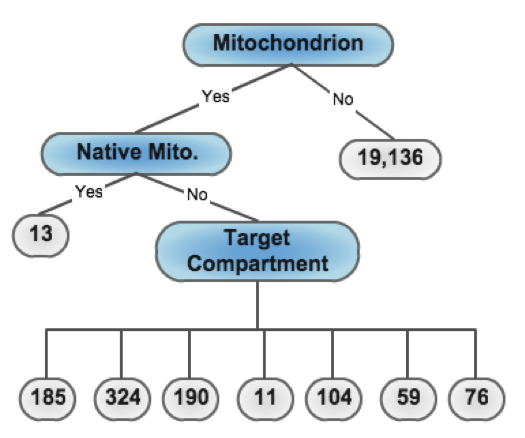
\includegraphics[width=0.75\columnwidth]{fig/Mito_tree}
    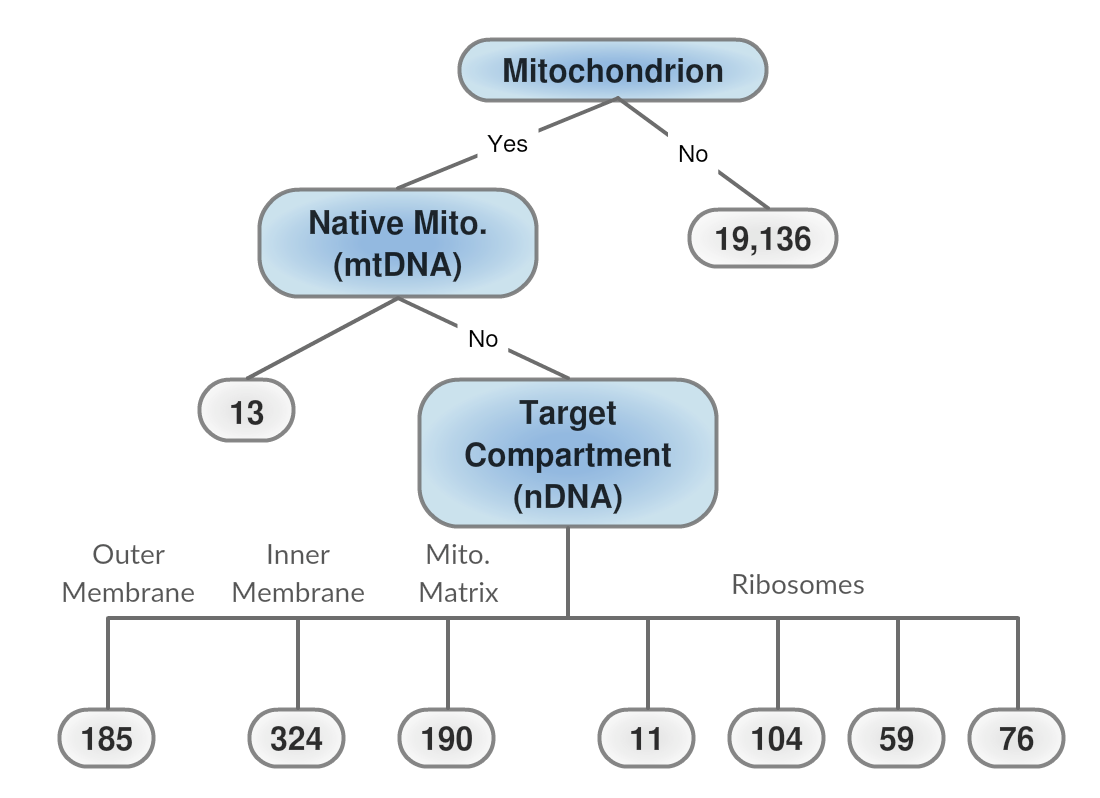
\includegraphics[width=0.75\columnwidth]{fig/MitoTreeLabels}
%        \caption{The protein dataset hierarchy of labels along with the instance
%        count for each label.}
        \label{fig:Mitotree}
    \end{figure}
\end{frame}
\begin{frame}
    \frametitle{Coarse-grained vs Fine-grained Trade Off}  % slide 13
    \framesubtitle{}
    \begin{figure}[!htb]
	\centering
    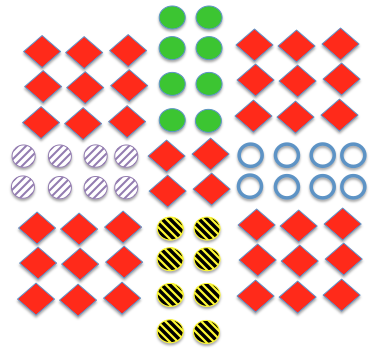
\includegraphics[width=0.6\columnwidth]{fig/union}
%    \caption{Demonstration of a dataset that would benefit from multiple fine-grained
%    learners for each circle type, from Mo et al.}
    \label{fig:union}
\end{figure}
\end{frame}
%\begin{frame}
%    \frametitle{Active Over-Labeling}  % slide 14
%    \framesubtitle{}
%    \begin{figure}[!htb]
%        \centering
%        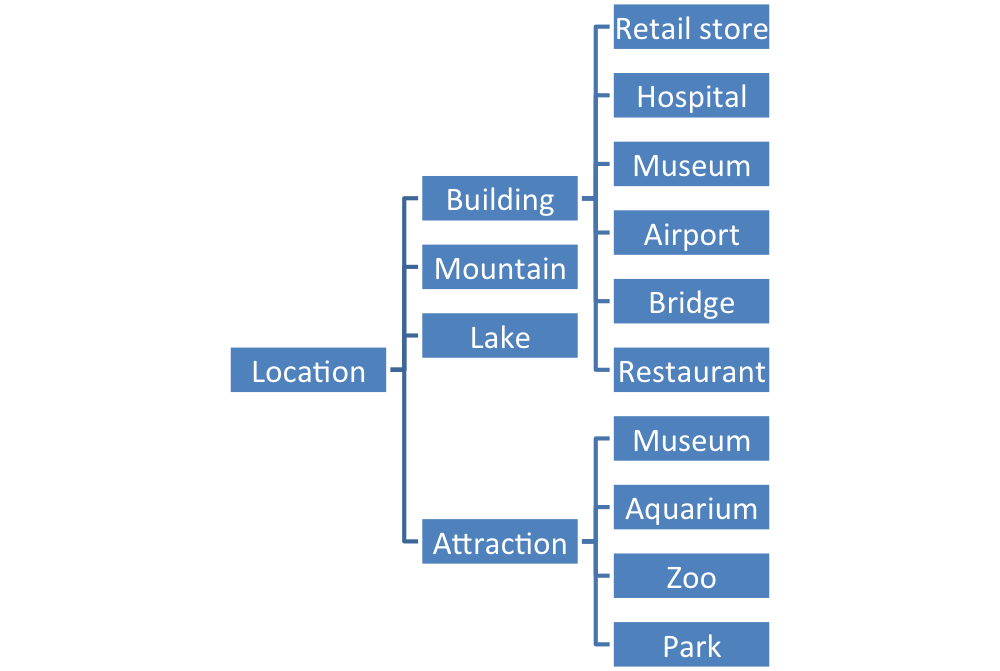
\includegraphics[width=0.85\columnwidth]{fig/exp-ontology}
%        \caption{A labeling tree based on the text categorization dataset RCV1, from Mo et al.}
%        \label{fig:exp-ontology}
%    \end{figure}
%\end{frame}
\begin{frame}
    \frametitle{Hierarchical Active Learning}  % slide 15
    \framesubtitle{}
    \par INPUT: purchase proportion $p$
    \begin{figure}[!htb]
        \centering
        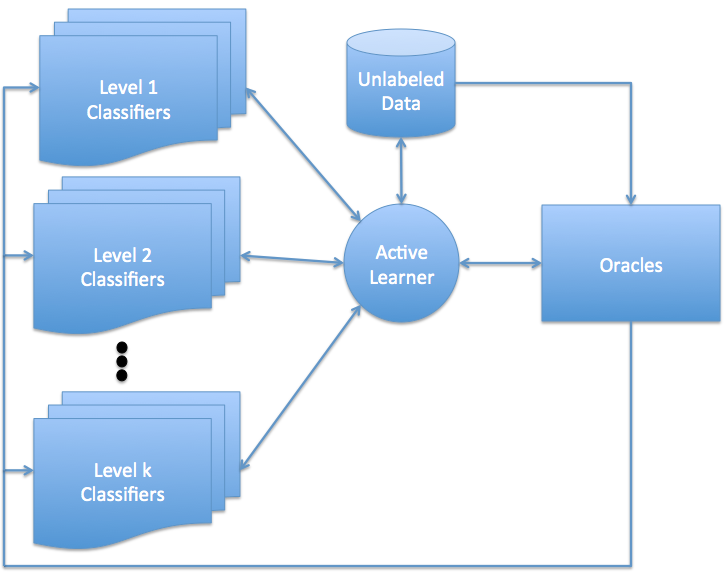
\includegraphics[width=0.65\columnwidth]{fig/AL2}
%        \caption{Diagram of HAL approach}
        \label{fig:HALapproach}
    \end{figure}
\end{frame}
\begin{frame}
    \frametitle{Dynamically Adapting Purchase Proportions}  % slide 16
    \framesubtitle{}
    \begin{figure}[!htb]
        \centering
        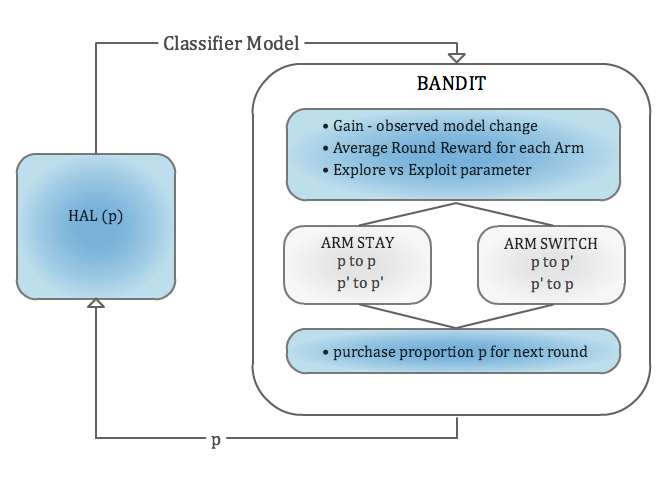
\includegraphics[width=1.0\columnwidth]{fig/BANDIT}
        \label{fig:BANDIT}
    \end{figure}
\end{frame}








%\section{Related Work}
%%\begin{frame}
%%    \frametitle{Related Work}
%%    \framesubtitle{}
%%    \begin{itemize}
%%      \item The experiments and methods described in this work
%%demonstrate how leveraging fine-grained label  information
%%can improve the accuracy of a coarse-grained (root-level) classifier, and
%% investigate active learning in a hierarchical setting where
%% label acquisition cost can vary, from Mo et al.
%%    \end{itemize}
%%\end{frame}
%\begin{frame}
%    \frametitle{Application to Dispatch Dataset}  % slide 17
%    \framesubtitle{}
%    \par Analysis and evaluation follow Mo et al.'s work.
%    \begin{itemize}
%      \item Fine outperforms Coarse in PR-AUC
%      \item Active outperforms Passive in PR-AUC
%      \item HAL ran with variable cost, fine proportions and budget
%      \item BANDIT approach shown to be robust to changes in cost and budget
%    \end{itemize}
%\end{frame}








\section{Exp. Setup}
\begin{frame}
    \frametitle{Training and Testing Coarse-Grain
    and Fine-Grain Classifiers}  % slide 18
    \framesubtitle{}
    \par Number of proteins in each class:
    \begin{table}[H]
      \centering
        %\caption{Class Totals}
        \label{tab:ClassesAll}
      \begin{tabular}{|l|l||l|}\hline
        Classes & Count & Totals \\ \hline
       Non Mito 0 & 19136 & All: 20098 \\
       mtDNA 1 & 13 & Coarse: 19136 \\
       nDNA 2 & 185 & Fine: 962 \\
       nDNA 3 & 324 & Features: 449 \\
       nDNA 4 & 190 & \\
       nDNA 5 & 11 &  \\
       nDNA 6 & 104  & \\
       nDNA 7 & 59  & \\
       nDNA 8 & 76  & \\ \hline
%        Tot All & 20098 \\
%        Tot Coarse & 19136 \\
%        Tot Fine & 962 \\
%        Features & 449 \\ \hline
      \end{tabular}%}
    \end{table}
\end{frame}
%\begin{frame}
%    \frametitle{Training and Testing Coarse-Grain
%    and Fine-Grain Classifiers}  % slide 19
%    \framesubtitle{}
%    \begin{table}[H]
%      \centering
%        \caption{Number of proteins in each partition:}
%        \label{tab:partitions}
%        \resizebox{1.0\columnwidth}{!}{%
%        \begin{tabular}{|l||l||l||l||l||l||l||l||l||l||l|}\hline
%    %    Folds & \multicolumn{9}{c}{Classes} \\ \cmidrule(r){2-11}
%        Folds & All & 0 & 1 & 2 & 3 & 4 & 5 & 6 & 7 & 8 \\ \hline
%        1 & 2010 & 1914 & 1 & 19 & 32 & 19 & 1 & 11 & 6 & 7 \\
%        2 & 2010 & 1914 & 1 & 19 & 32 & 19 & 1 & 11 & 6 & 7 \\
%        3 & 2010 & 1914 & 1 & 19 & 32 & 19 & 1 & 11 & 5 & 8 \\
%        4 & 2010 & 1914 & 1 & 19 & 32 & 19 & 1 & 10 & 6 & 8 \\
%        5 & 2010 & 1914 & 1 & 18 & 33 & 19 & 1 & 10 & 6 & 8 \\
%        6 & 2010 & 1914 & 1 & 18 & 33 & 19 & 1 & 10 & 6 & 8 \\
%        7 & 2010 & 1913 & 2 & 18 & 33 & 19 & 1 & 10 & 6 & 8 \\
%        8 & 2010 & 1913 & 2 & 18 & 33 & 19 & 1 & 10 & 6 & 8 \\
%        9 & 2009 & 1913 & 2 & 18 & 32 & 19 & 2 & 10 & 6 & 7 \\
%        10 & 2009 & 1913 & 1 & 19 & 32 & 19 & 1 & 11 & 6 & 7 \\ \hline
%        Total & 20098 & 19136 & 13 & 185 & 324 & 190 & 11 & 104 & 59 & 76 \\
%     \hline
%      \end{tabular}}
%    \end{table}
%\end{frame}
%\begin{frame}
%    \frametitle{Training and Testing Coarse-Grain and Fine-Grain Classifiers}  % slide 20
%    \framesubtitle{}
%     \par The following variables were varied for both SVM and Logit classifiers:
%    \begin{itemize}
%      \item Preprocessing Scaling Methods
%      \item Preprocessing Feature Selection
%      \item Class Weight
%      \item SVM Kernel, Cost, and Gamma parameters
%      \item Logit Cost, Fine class weights, Tolerance
%    \end{itemize}
%\end{frame}






\section{Conv. ML}
%\begin{frame}
%    \frametitle{SVM and Logit Classifier Performance}  % slide 21
%    \framesubtitle{Conventional ML}
%    \begin{table}[H]
%    \centering
%    \caption{Logit results after parameter tuning:}
%    \label{tab:LogRegAll-Wt23}
%    \resizebox{0.9\columnwidth}{!}{%
%    \begin{tabular}{|l||l||l||l||l||l||l|} \hline
%    Title & PR & ROC & Acc & F1 & conf (tn/fn) & conf (fp/tp) \\ \hline
%    coarse & 0.870 & 0.871 & 0.787 & 0.268 & ( 1503.2 / 17.8 ) & ( 410.4 / 78.3 ) \\
%    fine & 0.875 & 0.871 & 0.913 & 0.403 & ( 1776.5 / 37.3 ) & ( 137.1 / 58.8 ) \\ \hline
%    \end{tabular}
%    }
%    \end{table}
%    \begin{table}[H]
%    \centering
%    \caption{SVM results after parameter tuning:}
%    \label{tab:SVM-All}
%    \resizebox{0.9\columnwidth}{!}{%
%    \begin{tabular}{|l||l||l||l||l||l||l|}\hline
%    Title & PR & ROC & Acc & F1 & conf (tn/fn) & conf (fp/tp) \\ \hline
%    coarse & 0.892 & 0.880 & 0.866 & 0.347 & ( 1669.5 / 24.8 ) & ( 244.1 / 71.3 ) \\
%    fine & 0.898 & 0.882 & 0.942 & 0.485 & ( 1839.0 / 41.5 ) & ( 74.6 / 54.6 ) \\ \hline
%    \end{tabular}
%    }
%    \end{table}
%\end{frame}
\begin{frame}
    \frametitle{SVM and Logit Classifier Performance}  % slide 22
    \framesubtitle{F-measure Analysis}
    \begin{figure}[!htb]
        \centering
        \begin{subfigure}[t]{0.475\textwidth}
            \centering
            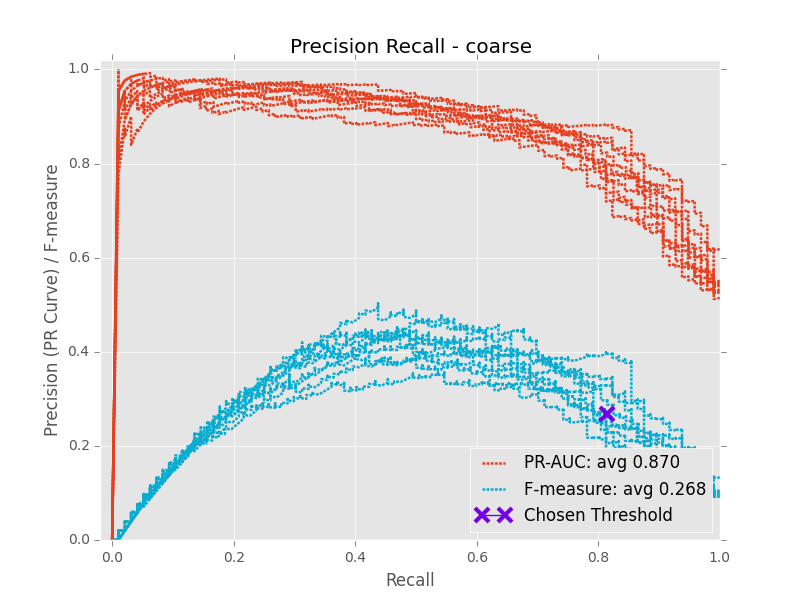
\includegraphics[width=\textwidth]{fig/LogReg_FindThreshold_PrCurve_coarse}
            \caption{Log Reg Pr Curves - Coarse}
        \end{subfigure}
        ~
        \begin{subfigure}[t]{0.475\textwidth}
            \centering
            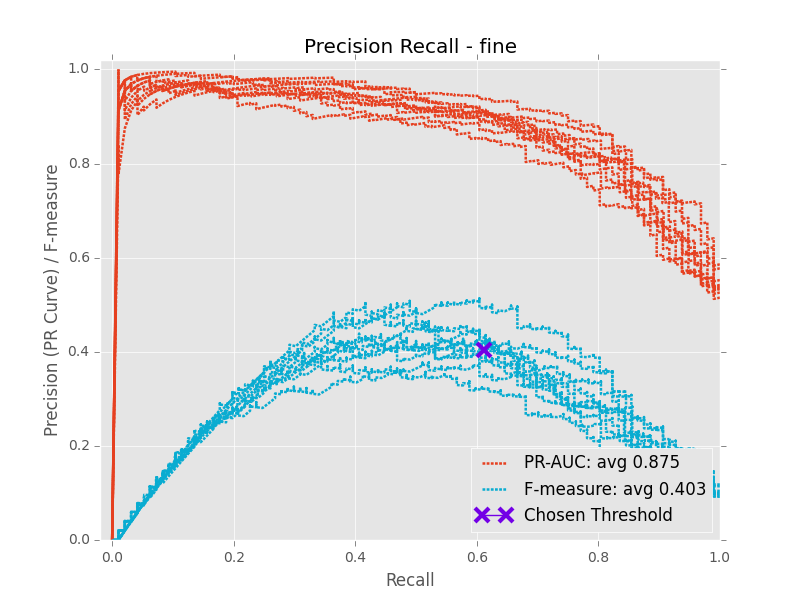
\includegraphics[width=\textwidth]{fig/LogReg_FindThreshold_PrCurve_fine}
            \caption{Log Reg Pr Curves - Fine}
        \end{subfigure}
%        \caption{The fine default threshold occurs at a point on the PR curve associated with a higher
%        F-measure score compared to the coarse curves.}
        \label{fig:LogRegThreshPr}
    \end{figure}
\end{frame}
\begin{frame}
    \frametitle{SVM and Logit Classifier Performance}  % slide 23
    \framesubtitle{F-measure Analysis}
    \begin{figure}[!htb]
        \centering
        \begin{subfigure}[t]{0.475\textwidth}
            \centering
            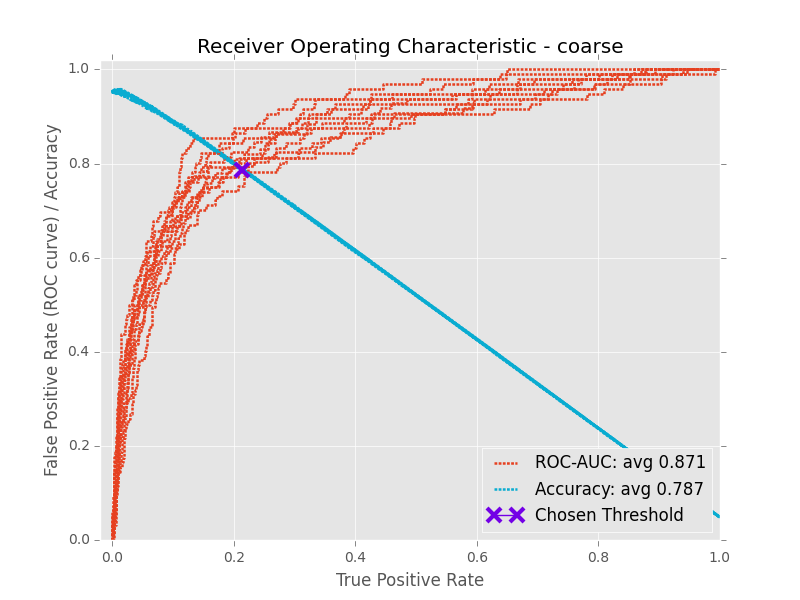
\includegraphics[width=\textwidth]{fig/LogReg_FindThreshold_RocCurve_coarse}
            \caption{Log Reg ROC Curves - coarse}
        \end{subfigure}%
        ~
        \begin{subfigure}[t]{0.475\textwidth}
            \centering
            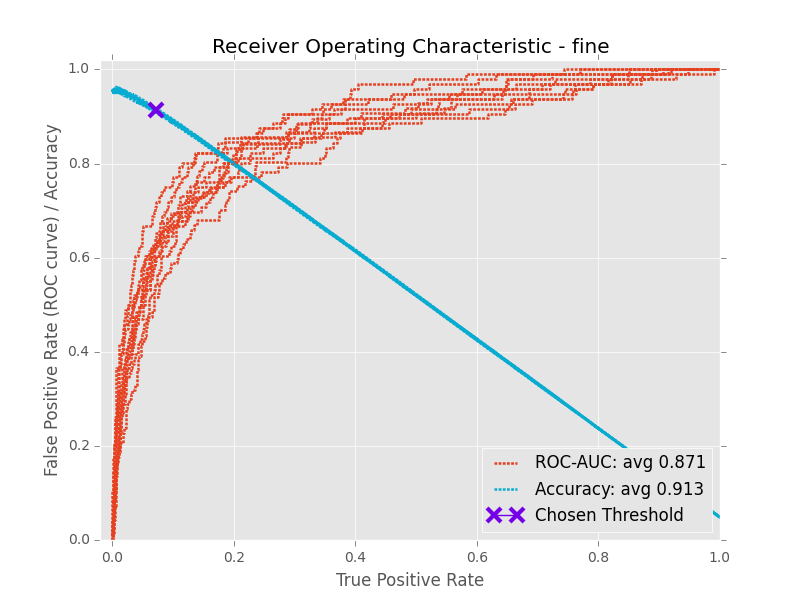
\includegraphics[width=\textwidth]{fig/LogReg_FindThreshold_RocCurve_fine}
            \caption{Log Reg ROC Curves - fine}
        \end{subfigure}
%        \caption{Fine has a higher accuracy than coarse at the default threshold for the Logit classifier.}
        \label{fig:LogRegThreshAcc}
    \end{figure}
\end{frame}







\section{Act. vs Pass.}
\begin{frame}
    \frametitle{Active vs. Passive Curve Analysis}  % slide 24
    \framesubtitle{Logit PR-AUC curves}
    \begin{figure}[!htb]
        \centering
        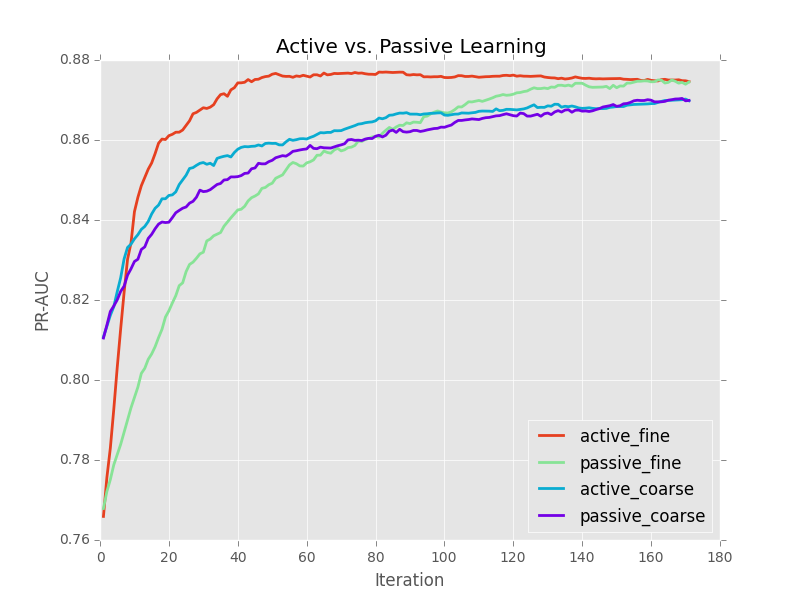
\includegraphics[width=0.80\columnwidth]{fig/runActPassLogReg_pr}
%        \caption{The PR-AUC curves for rounds with the Logit classifier conforms to expectations}
%    , with zactive fine having
%    the best performance, and active outperforming passive for both coarse
%    and fine classifier types.}
    \label{fig:runActPassLogReg_pr}
    \end{figure}
\end{frame}
\begin{frame}
    \frametitle{Active vs. Passive Curve Analysis}  % slide 25
    \framesubtitle{Logit ROC-AUC curves}
    \begin{figure}[!htb]
        \centering
        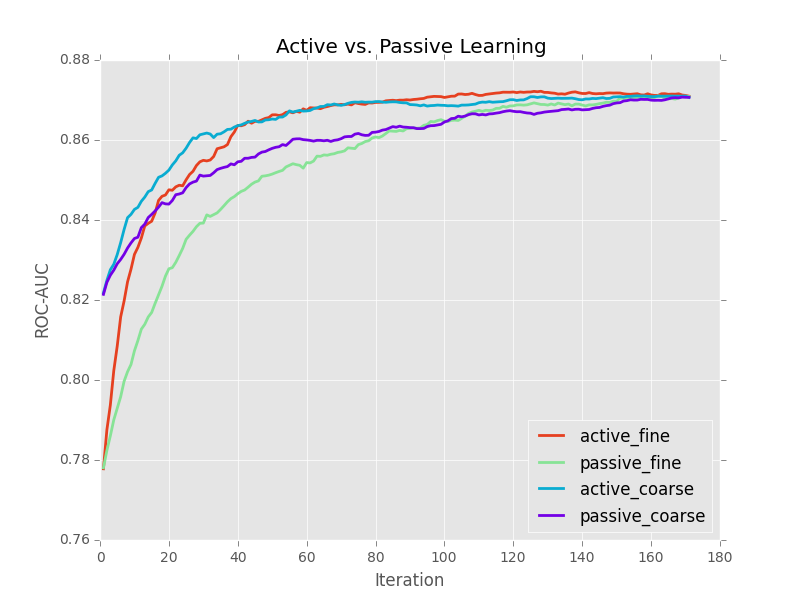
\includegraphics[width=0.80\columnwidth]{fig/runActPassLogReg_roc}
%        \caption{The ROC-AUC curves for rounds with the
%    Logit classifier; active curves beat out the passive
%    curves for both coarse and fine.}
%    Note that active fine ROC curve doesn't
%    converge to the active coarse ROC curve until round 40. This is contrasted
%    to a dominance of the active fine PR curve after round 10.}
    \label{fig:runActPassLogReg_roc}
    \end{figure}
\end{frame}
\begin{frame}
    \frametitle{Active vs. Passive Curve Analysis}  % slide 26
    \framesubtitle{SVM PR-AUC curves}
    \begin{figure}[!htb]
        \centering
        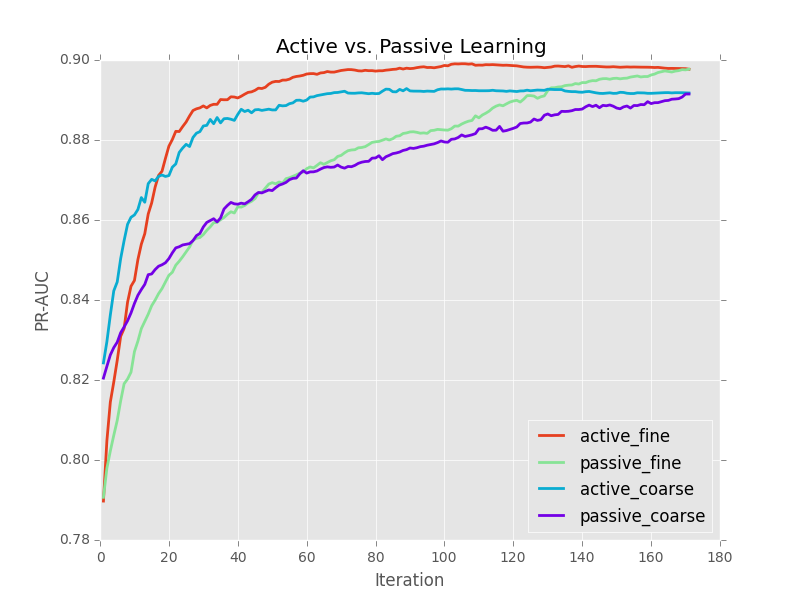
\includegraphics[width=0.80\columnwidth]{fig/runActPassSVM_pr}
        \label{fig:ActiveVsPassivePRSVM}
%        \caption{The PR AUC curves for SVM show a slight advantage for active fine,
%         similar to the Logit results.}
    \end{figure}
\end{frame}
\begin{frame}
    \frametitle{Active vs. Passive Curve Analysis}  % slide 27
    \framesubtitle{SVM ROC-AUC curves}
    \begin{figure}[!htb]
        \centering
        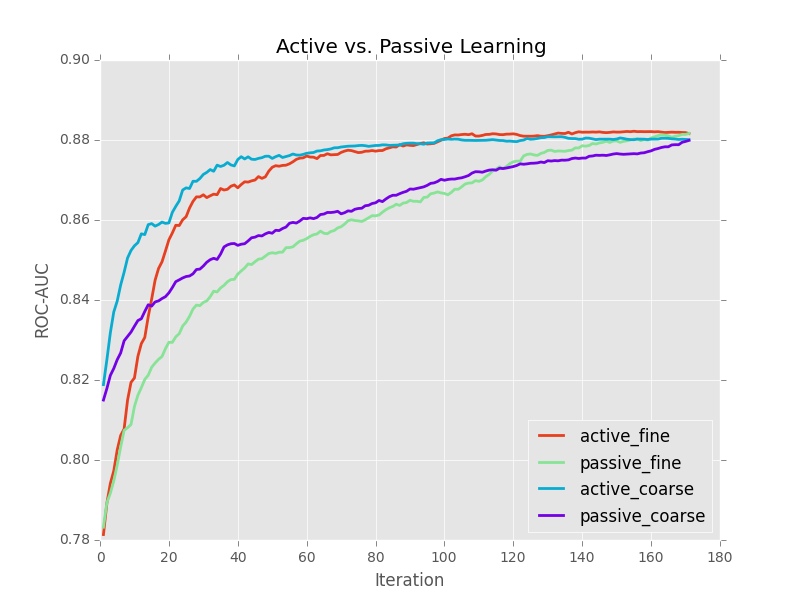
\includegraphics[width=0.80\columnwidth]{fig/runActPassSVM_roc}
        \label{fig:ActiveVsPassiveROCSVM}
%        \caption{The ROC AUC curves for SVM match the Logit results, the convergence of
%         active fine to active coarse takes slightly longer.}% , round 60 compared to round 40.}
    \end{figure}
\end{frame}








\section{HAL Results}
\begin{frame}
    \frametitle{Plots for Fine Fixed Ratio Results}  % slide 28
    \framesubtitle{Fine Cost 1}
    \begin{figure}[!htb]
	\centering
    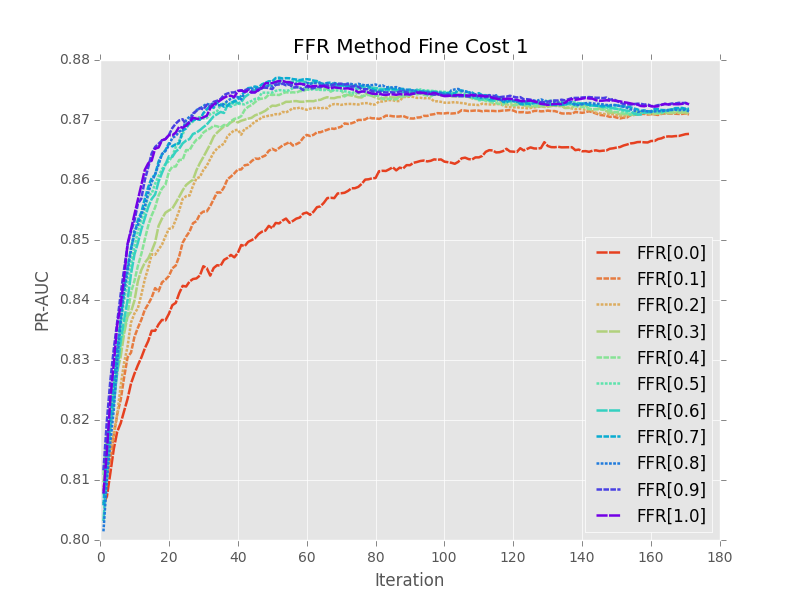
\includegraphics[width=0.8\columnwidth]{fig/ParamsFFR_PR_Cost1_rnds0_180}
%    \caption{The fine and coarse grain labels
%    both have a cost of 1.}
%    The purple 1.0 curve shows that if only fine-grained labels
%    are purchased, the highest performing PR-AUC can be obtained. All FFR ratios end at the same round
%    since the cost of the fine and coarse instances is the same the budget.}
%    \label{fig:ParamsFFR_PR_Cost1_rnds0_180}
\end{figure}
\end{frame}
\begin{frame}
    \frametitle{Plots for Fine Fixed Ratio Results}  % slide 29
    \framesubtitle{Fine Cost 2}
    \begin{figure}[!htb]
        \centering
        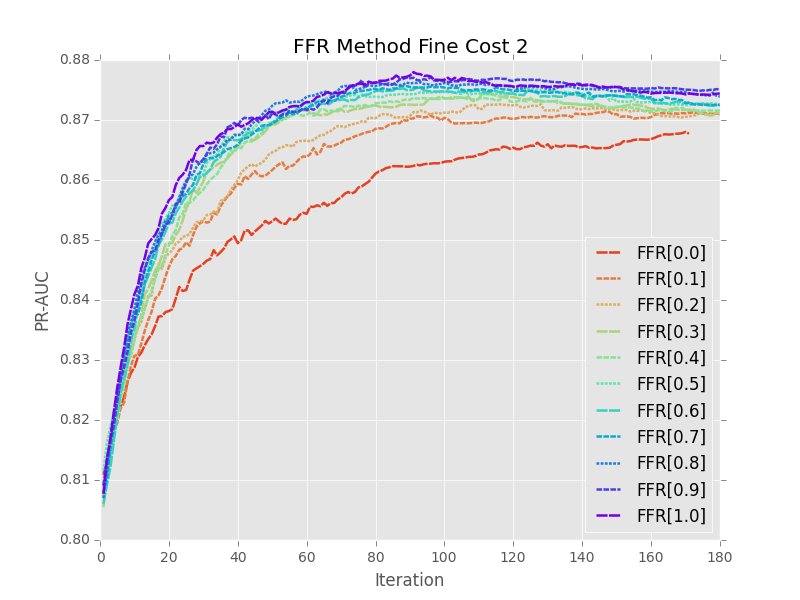
\includegraphics[width=0.8\columnwidth]{fig/ParamsFFR_PR_Cost2_rnds0_180}
%        \caption{At fine cost 2, advantage of the higher FFR values decreases but the ordering
%        of the curves remains unchanged.}
        \label{fig:ParamsFFR_PR_Cost2_rnds0_180}
    \end{figure}
\end{frame}
\begin{frame}
    \frametitle{Plots for Fine Fixed Ratio Results}  % slide 30
    \framesubtitle{Fine Cost 4}
    \begin{figure}[!htb]
        \centering
        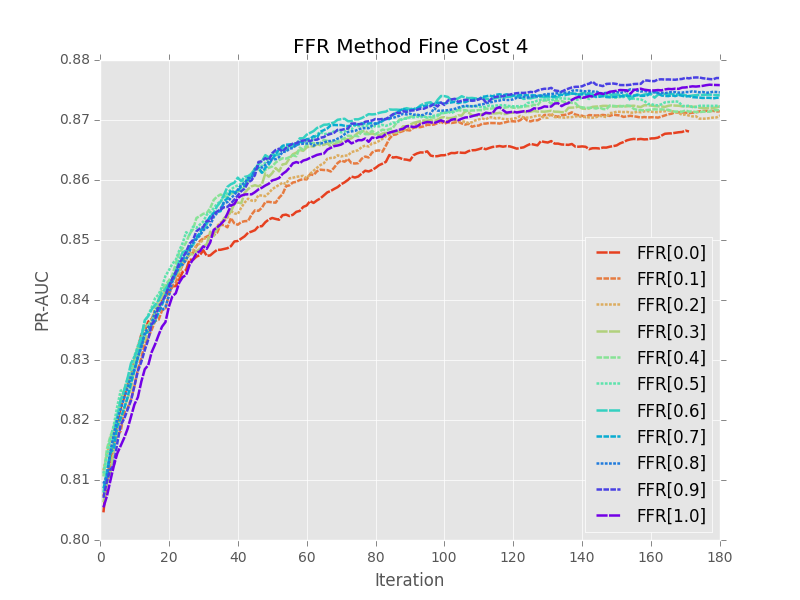
\includegraphics[width=0.8\columnwidth]{fig/ParamsFFR_PR_Cost4_rnds0_180}
%        \caption{At fine cost 4, the highest FFR $1.0$ is no longer preferred.
%Purchasing a greater number of coarse instances is a better strategy.}
%        , the
%        cost is to high for fine instances PR-AUC utility to overcome the PR-AUC
%        increase gained by purchasing more coarse instances.}
        \label{fig:ParamsFFR_PR_Cost4_rnds0_180}
    \end{figure}
\end{frame}
\begin{frame}
    \frametitle{Plots for Fine Fixed Ratio Results}  % slide 31
    \framesubtitle{Fine Cost 8}
    \begin{figure}[!htb]
        \centering
        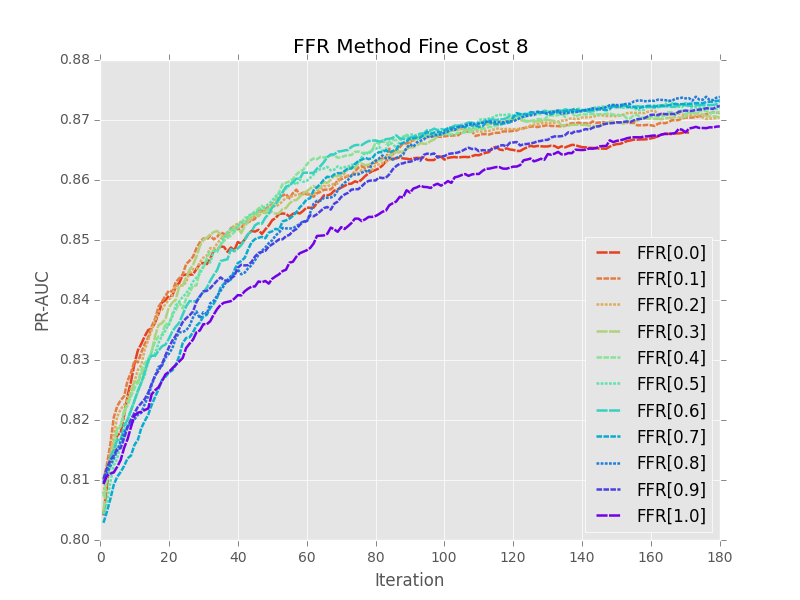
\includegraphics[width=0.8\columnwidth]{fig/ParamsFFR_PR_Cost8_rnds0_180}
%        \caption{At fine cost 8 the middle FFR values outperform the extreme values
%        for rounds 0 to 180.}
        \label{fig:ParamsFFR_PR_Cost8_rnds0_180}
    \end{figure}
\end{frame}
\begin{frame}
    \frametitle{Plots for Fine Fixed Ratio Results}  % slide 32
    \framesubtitle{Fine Cost 8 - Rnds to 500}
    \begin{figure}[!htb]
        \centering
        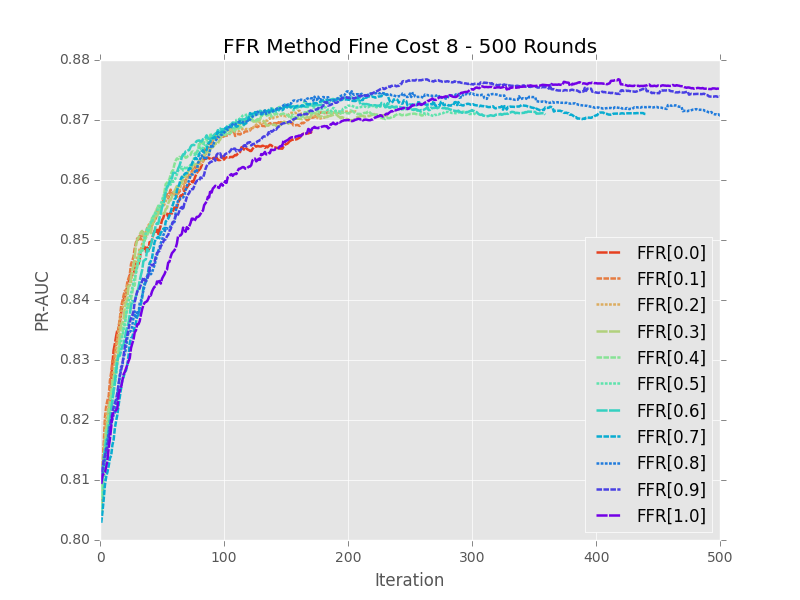
\includegraphics[width=0.8\columnwidth]{fig/ParamsFFR_PR_Cost8_rnds0_500}
%        \caption{This shows the iterations continuing through round 500, the curves
%        with the higher fine rates settle to the same end point.}
%         that the
%        curves with the high rates of coarse labels purchased achieved at previous
%        iterations.}
        \label{fig:ParamsFFR_PR_Cost8_rnds0_500}
    \end{figure}
\end{frame}
\begin{frame}
    \frametitle{Plots for Fine Fixed Ratio Results}  % slide 33
    \framesubtitle{Fine Cost 8 - Rnds 20 to 60}
    \begin{figure}[!htb]
        \centering
        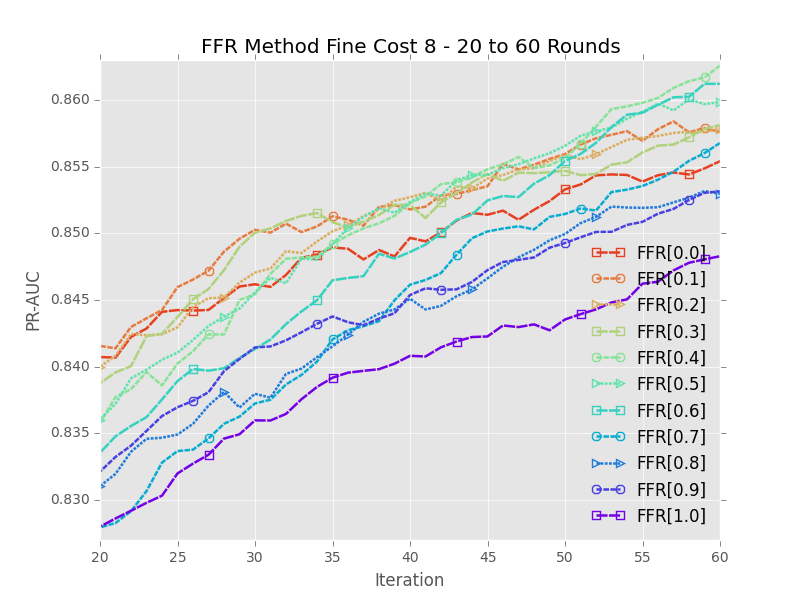
\includegraphics[width=0.8\columnwidth]{fig/ParamsFFR_PR_Cost8_rnds20_60}
%        \caption{The fine cost 8 curves shown expanding the rounds 20-60. If a round budget of 40
%        occurs than the recommended FFR would be $0.2$.}
        \label{fig:ParamsFFR_PR_Cost8_rnds20_60}
    \end{figure}
\end{frame}
\begin{frame}
    \frametitle{Plots for Fine Fixed Ratio Results}  % slide 34
    \framesubtitle{Fine Cost 16}
    \begin{figure}[!htb]
        \centering
        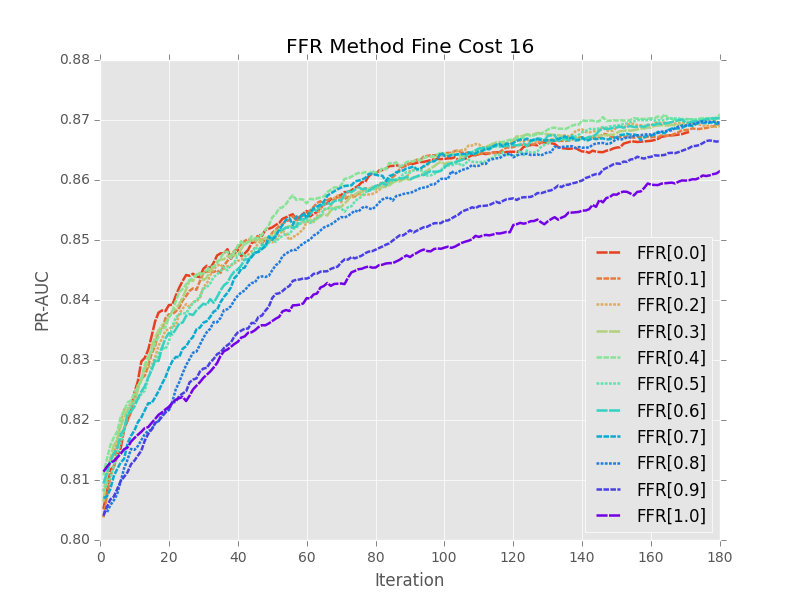
\includegraphics[width=0.8\columnwidth]{fig/ParamsFFR_PR_Cost16_rnds0_180}
        \caption{The fine cost is increased to 16. The fine cost is to high to offset the decreased number of instances purchased.}
%        The cost is to high for the fine label advantage to offset
%        the decreased number of instances purchased.}
        \label{fig:ParamsFFR_PR_Cost16_rnds0_180}
    \end{figure}
\end{frame}









\section{BANDIT Results}
\begin{frame}
    \frametitle{BANDIT Approach Results}  % slide 35
    \framesubtitle{Varying Cost Analysis}
    \begin{figure}[!htb]
        \begin{itemize}
      \item The BANDIT approach is compared to the previous FFR curves for the
      following fine-grain costs $\{1.0, 1.1, 1.2, 1.5, 2.0, 4.0, 8.0, 16.0, 32.0, 64.0\}$
      \item Budget held fixed at round 120.
      \item The metric \textit{diff} is the learner's absolute difference
     in PR-AUC from the top learner for a given cost.
     \item The metric \textit{rank} is the learners
     $0$ indexed ranking in terms of PR-AUC for a given cost.
    \end{itemize}
    \end{figure}
\end{frame}
\begin{frame}
    \frametitle{BANDIT Approach Results}  % slide 36
    \framesubtitle{Varying Cost Analysis - Plot}
    \begin{figure}[!htb]
        \centering
        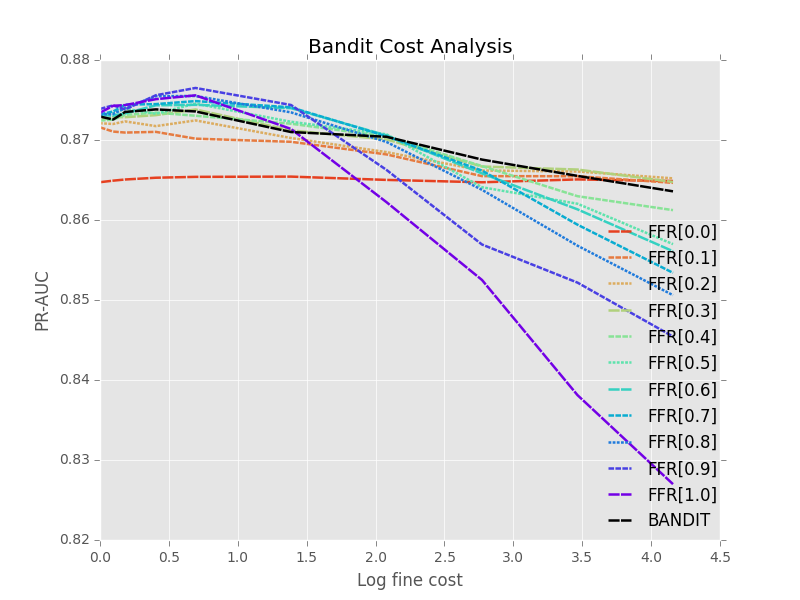
\includegraphics[width=0.80\columnwidth]{fig/BanditPlotLogFine}
%        \caption{BANDIT log fine cost analysis with budget fixed.}
        \label{fig:BanditPlotLogFine}
    \end{figure}
\end{frame}
\begin{frame}
    \frametitle{BANDIT Approach Results}  % slide 37
    \framesubtitle{Varying Cost Analysis - Rank and Diff Metrics}
        \begin{table}[H]
%        \caption{Aggregated PR AUC for the protein dataset}
        \centering
        \resizebox{0.9\columnwidth}{!}{%
        \begin{tabular}{lrrrrrrrr}
        \hline
        {} &  diff &       &       &       & rank &     &        &       \\
        {} &   min &   max &  mean &   std &  min & max &   mean &   std \\
        \hline
        algorithm &       &       &       &       &      &     &        &       \\
        BANDIT & 0.000 & 0.003 & \underline{\textbf{0.001}} & 0.001 & 0 & 8 & 4.8 & 2.315 \\
        FFR[$0.0$] & 0.000 & 0.011 & 0.007 & 0.004 & 1 & 11 & 8.8 & 3.429 \\
        FFR[$0.1$] & 0.001 & 0.006 & 0.003 & 0.002 & 3 & 10 & 8.0 & 2.793 \\
        FFR[$0.2$] & 0.000 & 0.004 & 0.002 & 0.001 & 0 & 9 & 6.5 & 3.500 \\
        FFR[$0.3$] & 0.000 & 0.003 & 0.001 & 0.001 & 0 & 8 & 5.1 & 2.663 \\
        FFR[$0.4$] & 0.000 & 0.004 & 0.002 & 0.001 & 1 & 8 & 5.6 & 2.200 \\
        FFR[$0.5$] & 0.000 & 0.008 & 0.002 & 0.002 & 0 & 8 & 4.6 & 2.200 \\
        FFR[$0.6$] & 0.000 & 0.009 & 0.002 & 0.003 & 1 & 7 & 4.6 & 1.855 \\
        FFR[$0.7$] & 0.000 & 0.012 & 0.002 & 0.004 & 0 & 8 & \underline{\textbf{3.3}} & 2.571 \\
        FFR[$0.8$] & 0.000 & 0.015 & 0.003 & 0.005 & 1 & 9 & 4.8 & 3.027 \\
        FFR[$0.9$] & 0.000 & 0.020 & 0.005 & 0.007 & 0 & 10 & 4.3 & 4.605 \\
        FFR[$1.0$] & 0.000 & 0.038 & 0.009 & 0.013 & 1 & 11 & 5.6 & 4.630 \\
        \hline
        \end{tabular}}
        \label{tab:banditLogFine}
        \end{table}
\end{frame}
\begin{frame}
    \frametitle{BANDIT Approach Results}  % slide 38
    \framesubtitle{Varying Budget Analysis - Mixed Cost}
    \begin{figure}[!htb]
        \centering
        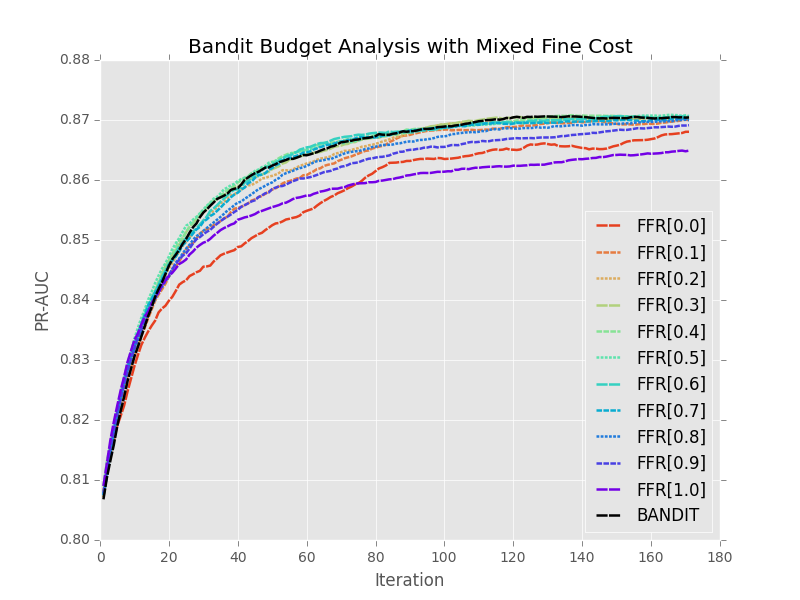
\includegraphics[width=0.80\columnwidth]{fig/BanditMixedCostPR}
%        \caption{BANDIT mixed fine cost plot.}
        \label{fig:BanditMixedCostPR}
    \end{figure}
\end{frame}
\begin{frame}
    \frametitle{BANDIT Approach Results}  % slide 39
    \framesubtitle{BANDIT - Rnds 20 to 60}
    \begin{figure}[!htb]
        \centering
        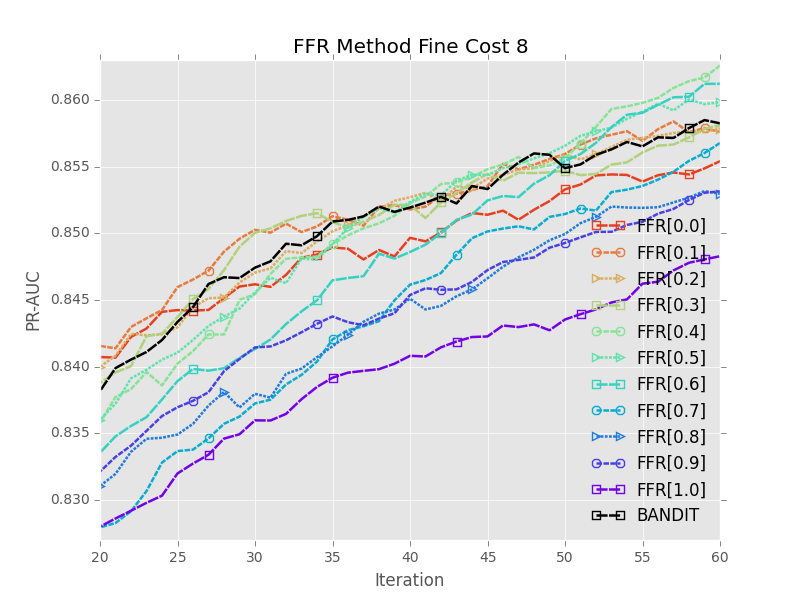
\includegraphics[width=0.80\columnwidth]{fig/BANDIT_PR_Cost8_rnds20_60}
%        \caption{
%        The fine cost 8 curves shown expanding the rounds 20-60. With the BANDIT approach
%        plotted.
%%        At budget iteration 40, BANDIT PR-AUC is within $0.0007$ of the top learner's
%%        PR-AUC.
%        }
        \label{fig:BANDIT_PR_Cost8_rnds20_60}
    \end{figure}
\end{frame}







\section{Conclusions}
\begin{frame}
    \frametitle{Conclusions}  % slide 40
    \framesubtitle{}
    \begin{itemize}
    \item Demonstrated fine-grained labels can be used to improve a coarse-grained classifier for the protein dataset
    \item Demonstrated a prominent advantage for active fine with the Logit classifier
    \item HAL is implemented and applied to the protein dataset for various FFR proportions and fine label costs
    \item The BANDIT approach is shown to be robust to both labeling cost and budget
    \end{itemize}
\end{frame}
\begin{frame}
    \frametitle{Future Work}  % slide 41
    \framesubtitle{}
    \begin{itemize}
      \item Future work is to apply the active over-labeling approach
      to other datasets with more complex hierarchical label trees;
      datasets derived from Gene Ontology research could be investigated
    \end{itemize}
\end{frame}
\begin{frame}
    \frametitle{Acknowledgements}
    \framesubtitle{}
    \begin{itemize}
      \item I would like to thank my advisor Dr. Stephen Scott,
      Yugi Mo and Dr. Douglas Downey for continued guidance. I would like to
      thank Dr. Juan Cui and Dr. Ashok Samal for serving on my comittee. Additionally,
      I would like to thank Jiang Shu and Kevin Chiang for their
      assistance accessing and understanding the protein dataset.
    \end{itemize}
\end{frame}
\begin{frame}
    \frametitle{Questions}  % slide 42
    \framesubtitle{jamesdduin@gmail.com}
    \begin{figure}[!htb]
        \centering
        
\includegraphics[width=1.0\columnwidth]{fig/question}
        \label{fig:question}
    \end{figure}
\end{frame}
\begin{frame}[noframenumbering]
    \frametitle{Active vs. Passive Curve Analysis}
    \framesubtitle{Logit Accuracy}
    \begin{figure}[!htb]
        \centering
        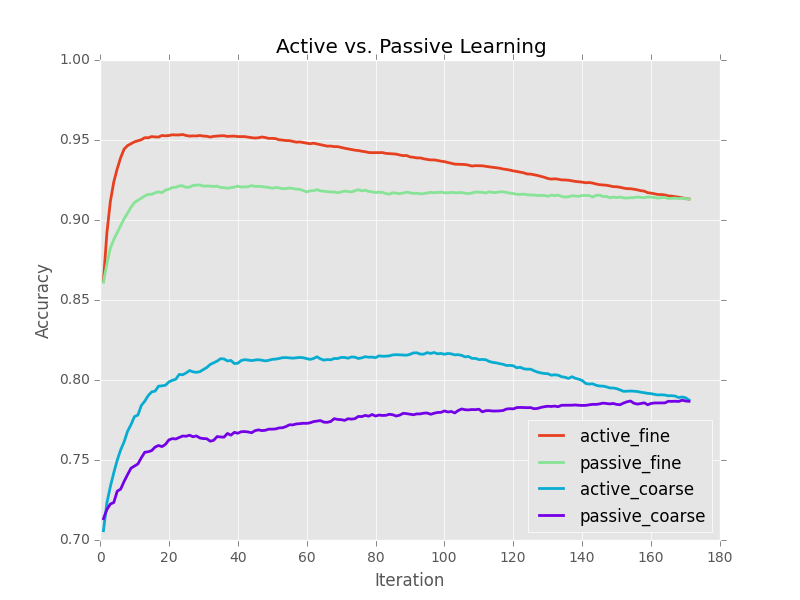
\includegraphics[width=0.80\columnwidth]{fig/runActPassLogReg_acc}
        \label{fig:runActPassLogReg_acc}
        \caption{The accuracy of the classifiers stays at
roughly the same rate throughout the rounds; this is due to an effective
weighting scheme.}
    \end{figure}
\end{frame}
\begin{frame}[noframenumbering]
    \frametitle{Active vs. Passive Curve Analysis}
    \framesubtitle{Logit F-measure}
    \begin{figure}[!htb]
        \centering
        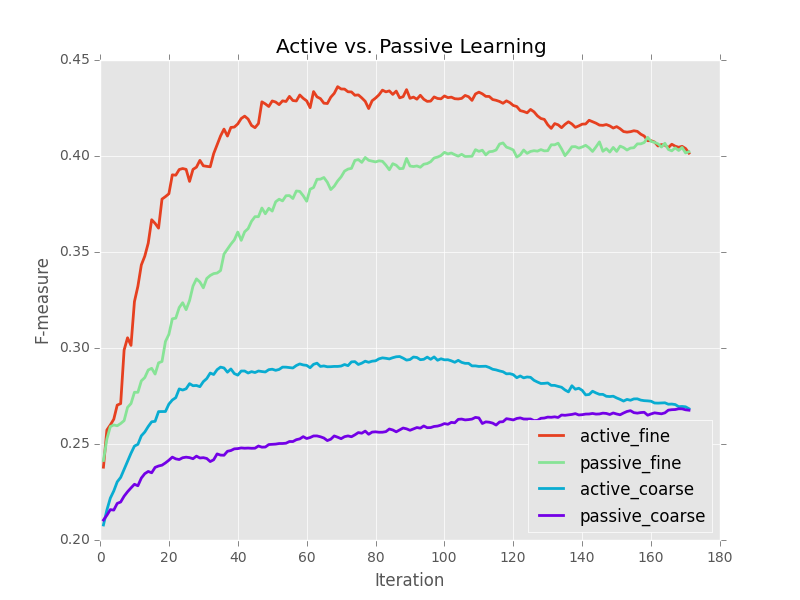
\includegraphics[width=0.70\columnwidth]{fig/runActPassLogReg_f1}
        \label{fig:runActPassLogReg_f1}
        \caption{Both curves show a dominance of fine over coarse and
Active over Passive.}
    \end{figure}
\end{frame}
\begin{frame}[noframenumbering]
    \frametitle{Dynamically Adapting Purchase Proportions $p$ or $p'$}  % slide 16
    \framesubtitle{}
\begin{itemize}
      \item For round $n$, calculate gain $g$ in terms of observed model change
      \item Calculate average round reward for each arm
      \item Calculate $\varepsilon_n= \min \left \{1,\frac{2}{n}  \right \}$
      \item With probability $1-\varepsilon_n$ play arm with highest current average reward for round $n$, otherwise explore
      \item After playing arm, run HAL with chosen $p$ or $p'$
    \end{itemize}
    \begin{table}[H]
      \centering
        %\caption{Class Totals}
        \label{tab:ClassesAll}
      \begin{tabular}{|l||l|}\hline
        ARM STAY & ARM SWITCH  \\ \hline
        $r(n) = 0$ &
        $r(n)=
            \begin{cases}
               -g(n)/|g(n)| & \text{if } p \rightarrow p'\\
                g(n)/|g(n)| & \text{if } p' \rightarrow p\\
                0 & \text{if }  p \rightarrow  p \text{ or }  p' \rightarrow p' \\
            \end{cases}$ \\ \hline
      \end{tabular}%}
    \end{table}
%    \begin{itemize}
%      \item HAL is a fixed-fine ratio (FFR) methodology
%      \item Input is a purchase proportion
%vector $p$, which allocates budget to purchase labels at a given level in the hierarchy %specifies how much of the budget should be
%      \item The task of choosing the
%level of granularity to purchase labels is solved using Auer et al.'s $\epsilon$-greedy bandit algorithm %framed as a multi-armed bandit problem, and
%\item With probability $1-\varepsilon_n$ play arm with highest current average reward for round $n$, otherwise explore
%    \end{itemize}
\end{frame}
%\section{Bibliography}
\begin{frame}[noframenumbering]
    \frametitle{Bibliography}
    \framesubtitle{}
    \begin{itemize}
      \item Y. Mo, S. D. Scott, and D. Downey, “Learning hierarchically decomposable concepts with active over-labeling,” in 2016 IEEE 16th International Conference on Data Mining (ICDM), Dec 2016, pp. 340–349.
      \item J. Z. Juan Cui, Kevin Chiang, “Prediction of nuclear and locally encoded mitochondrion.” Lincoln, NE: Nebraska Gateway to Nutrigenomics 6th Annual Retreat, June 9 2014. [Online]. Available: http://cehs.unl.edu/nutrigenomics/ nebraska-gateway-nutrigenomics-6th-annual-retreat/
      \item T. M. Mitchell, Machine Learning, 1st ed. New York, NY, USA: McGraw-Hill, Inc., 1997.
    \end{itemize}
\end{frame}
\begin{frame}[noframenumbering]
    \frametitle{Bibliography}
    \framesubtitle{}
    \begin{itemize}
      \item L. Buitinck, G. Louppe, M. Blondel, F. Pedregosa, A. Mueller, O. Grisel, V. Niculae, P. Prettenhofer, A. Gramfort, J. Grobler, R. Layton, J. VanderPlas, A. Joly, B. Holt, and G. Varoquaux, “API design for machine learning software: experiences from the scikit-learn project,” in ECML PKDD Workshop: Languages for Data Mining and Machine Learning, 2013, pp. 108–122
      \item D. Cotter, P. Guda, E. Fahy, and S. Subramaniam, “Mitoproteome: mitochondrial protein sequence database and annotation system,” Nucleic Acids Research, vol. 32, no. suppl1, p. D463, 2004. [Online]. Available: +http://dx.doi.org/10.1093/nar/gkh048
    \end{itemize}
\end{frame}
\begin{frame}[noframenumbering]
    \frametitle{Bibliography}
    \framesubtitle{}
    \begin{itemize}
      \item J. Cui, L. Y. Han, H. Li, C. Y. Ung, Z. Q. Tang, C. J. Zheng, Z. W. Cao, and Y. Z. Chen, “Computer prediction of allergen proteins from sequence-derived protein structural and physicochemical properties,” Molecular Immunology, vol. 44, no. 4, pp. 514 – 520, 2007. [Online]. Available: http://www.sciencedirect.com/science/article/pii/S0161589006000368
      \item A. McCallum, R. Rosenfeld, T. M. Mitchell, and A. Y. Ng, “Improving text classification by shrinkage in a hierarchy of classes,” in Proceedings of the Fifteenth International Conference on Machine Learning, ser. ICML ’98. San Francisco, CA, USA: Morgan Kaufmann Publishers Inc., 1998, pp. 359–367. [Online]. Available: http://dl.acm.org/citation.cfm?id=645527.657461
    \end{itemize}
\end{frame}
\begin{frame}[noframenumbering]
    \frametitle{Bibliography}
    \framesubtitle{}
    \begin{itemize}
      \item W. Jiang and Z. W. Ras, “Multi-label automatic indexing of music by cascade classifiers,” Web Intelli. and Agent Sys., vol. 11, no. 2, pp. 149–170, Apr. 2013. [Online]. Available: http://dl.acm.org/citation.cfm?id=2590084.2590088
      \item etc.
    \end{itemize}
\end{frame}






%\begin{frame}
%    \frametitle{Introduction}
%    \framesubtitle{}
%    \texttt{Beamer} is a wonderful \LaTeX\ document class that produces
%    high quality PDF slide presentations.
%    Moreover, you can customize and develop your own themes!
%\end{frame}


%\section{UNL Theme}
%\begin{frame}
%    \frametitle{UNL Theme}
%    \framesubtitle{}
%    This theme was developed for the University of Nebraska--Lincoln.
%    The theme itself was developed from the PaloAlto, sidebar and sidbartab
%    themes available by default in beamer.
%    However, this theme has several unique features and customizations:
%    \begin{itemize}
%      \item The color theme uses UNL's ``scarlet and creme'' colors.
%      \item Improved spacing.
%      \item Math mode preserves \LaTeX's serif font.
%      \item Incorporates UNL's Logo automatically.
%      \item Unique drop shadows on the top and side bars!
%    \end{itemize}
%\end{frame}
%
%
%\begin{frame}
%    \frametitle{Other Features}
%    \framesubtitle{}
%    For convenience, if you are in handout mode, all features, including the
%    navigation symbols at the bottom right are shut off!
%    Beamer boxes are by default, rounded and have a drop shadow.  All beamer
%    boxes (definition, theorem, etc) have the same color scheme.
%    \begin{definition}
%      This is my definition
%      $$A = \{p \mid \textrm{$p$ is prime }\}$$
%    \end{definition}
%    \begin{theorem}
%      The set $A$ is countable.
%    \end{theorem}
%\end{frame}
%
%

%\section{Using The Theme}
%\begin{frame}[fragile]
%    \frametitle{How To Use The Theme}
%    \framesubtitle{Theme Options}
%    To use the UNL Theme, after your document class declaration, simply use:
%    \begin{verbatim}\usetheme{UNLTheme}\end{verbatim}
%    To pass options to the package, use
%    \verb"\usetheme[left,hideothersubsections,width=2.5cm]{UNLTheme}"
%\end{frame}
%
%\begin{frame}[fragile]
%    \frametitle{How To Use The Theme}
%    \framesubtitle{Theme Options}
%    There are also several options that you can pass:
%    \begin{itemize}
%      \item \texttt{hideothersubsections} -- This hides subsections in the
%            sidebar \emph{other than} the subsections of the current section.
%      \item \texttt{hideallsubsections} -- This option doesn't print \emph{any}
%            subsections in the sidebar.
%      \item \texttt{width} -- sets the width of the sidebar, default is
%      	    \verb"2.5\baselineskip"
%      \item \texttt{height} -- sets the height of the header, default is
%      	    \verb"2.5\baselineskip"
%      \item \texttt{left} -- sets the sidebar to the left of the slide (default).
%      \item \texttt{right} -- sets the sidebar to the right of the slide.
%    \end{itemize}
%\end{frame}
%
%\begin{frame}
%    \frametitle{How To Get The Theme}
%    \framesubtitle{}
%    The theme is available from my home page,
%    \textcolor{blue}{\url{http://www.cse.unl.edu/~cbourke/}}
%    You need \texttt{You need beamerthemeUNLTheme.sty} and \texttt{UNL.pdf}
%    (the UNL logo).
%    Place them in the working directory or add them to \texttt{beamer/themes/theme}
%    or somewhere in your \LaTeX\ path and you're good to go!
%\end{frame}
    
\end{document}
